
\chapter*{Introduction}
\addstarredchapter{Introduction}

\chapter{État de l'art sur la détection de communautés et les réseaux dynamiques}
\minitoc
Au cours de cette thèse, nous étudions deux axes de recherches liés aux graphes qui sont orthogonaux.
D'une part, il s'agit de la détection de structures dans les graphes et plus particulièrement de communautés.
Un communauté est un sous-ensemble de n\oe uds de manière à ce qu'ils soient fortement connectés.
Il n'existe cependant aucune définition exact et la notion de communauté fortement connectée dépends du contexte et de la méthode.
Malgré cette définition floue, des structures communautaires ont été trouvées dans de nombreux graphes dans plusieurs domaines tel que les réseaux de dans le cerveau \cite{DeReus2014}, réseau d'eau \cite{DiNardo2015} , animaux \cite{Farine2015}\REF . \REF.
Ces notions de communautés et les méthodes de détection sont définies dans la section~\ref{sec:intro_communaute}.\\

D'autre part, il a été observé que la modélisation d'un réseau sous la forme d'un graphe peut poser problème notamment quand le réseau change au cours du temps \REF.
Face à ce problème plusieurs extensions de la théorie des graphes ont été proposées et elles sont résumées dans la section~\ref{sec:intro_extension_temporelle}.



\section{Communauté dans les graphes}
\label{sec:intro_communaute}

Ce champs de recherche est très vaste et il est illusoire de vouloir énumérer les méthodes existantes dans ce domaine car les caractéristiques voulues d'une communauté peuvent varier~\cite{Coscia2011,Leskovec2008,Yang2015,Jeub2015}.
Il y a tout de même deux grandes catégories qui permette de séparer les méthodes existantes.
Dans ces deux catégories, les méthodes existantes cherchent à capturer 
des communautés fortement connectées mais elles différent sur ce qu'elles capturent comme structures communautaires.
Les communautés d'une structure communautaires peuvent être disjointes, c'est-à-dire que deux communautés n'ont aucun n\oe uds en commun, ou alors recouvrantes, c'est-à-dire que deux communautés peuvent avoir plusieurs n\oe uds en commun.
Dans le premier cas, on parle de partition des n\oe uds et dans le second on parle de couverture ou partitions chevauchantes de n\oe uds.
Dans ces deux cas, il y a également une contrainte sur le fait que tout les n\oe uds doivent appartenir à au moins une communauté.
C'est deux structures sont correspondent à deux visions possibles de l'organisation d'un graphe et du réseau sous-jacent.
Nous présentons ces deux catégories dans les sous-sections suivantes.

\subsection{Parititons de n\oe uds}
Afin de mieux comprendre ce que peux capturer une parition de n\oe uds, il est plus facile de partir d'un exemple.
Dans l'étude de Stehlé~\emph{et al.}~\cite{Stehle2011}, des enfants d'une école primaire ont eu pendant 2 jours des capteurs enregistrant lorsque deux enfant sont à une distance de moins de 1m50 l'un de l'autre.
Ce dispositif permet de mesurer les interactions entre élèves et de construire le graphe des relations entre élève à l'école.
Une illustration du graphe obtenu est visible dans la figure~\ref{fig:ecole_primaire}.
La classe de chaque élève est également connue.
Comme chaque élève appartient à une et une seule classe, les classes forment une partition des élèves.
Cette partition est une bonne structure communautaire car on remarque que les élèves d'une même classe parle beaucoup entre eux mais ils parlent peu entre élèves de classes différentes.
Cela se remarque particulièrement bien pour la classe 3A.
Il existe beaucoup de liens entre les élèves de la classe 3A et aucun entre eux et les élèves de la classe 5A par exemple.

\begin{figure}
\centering
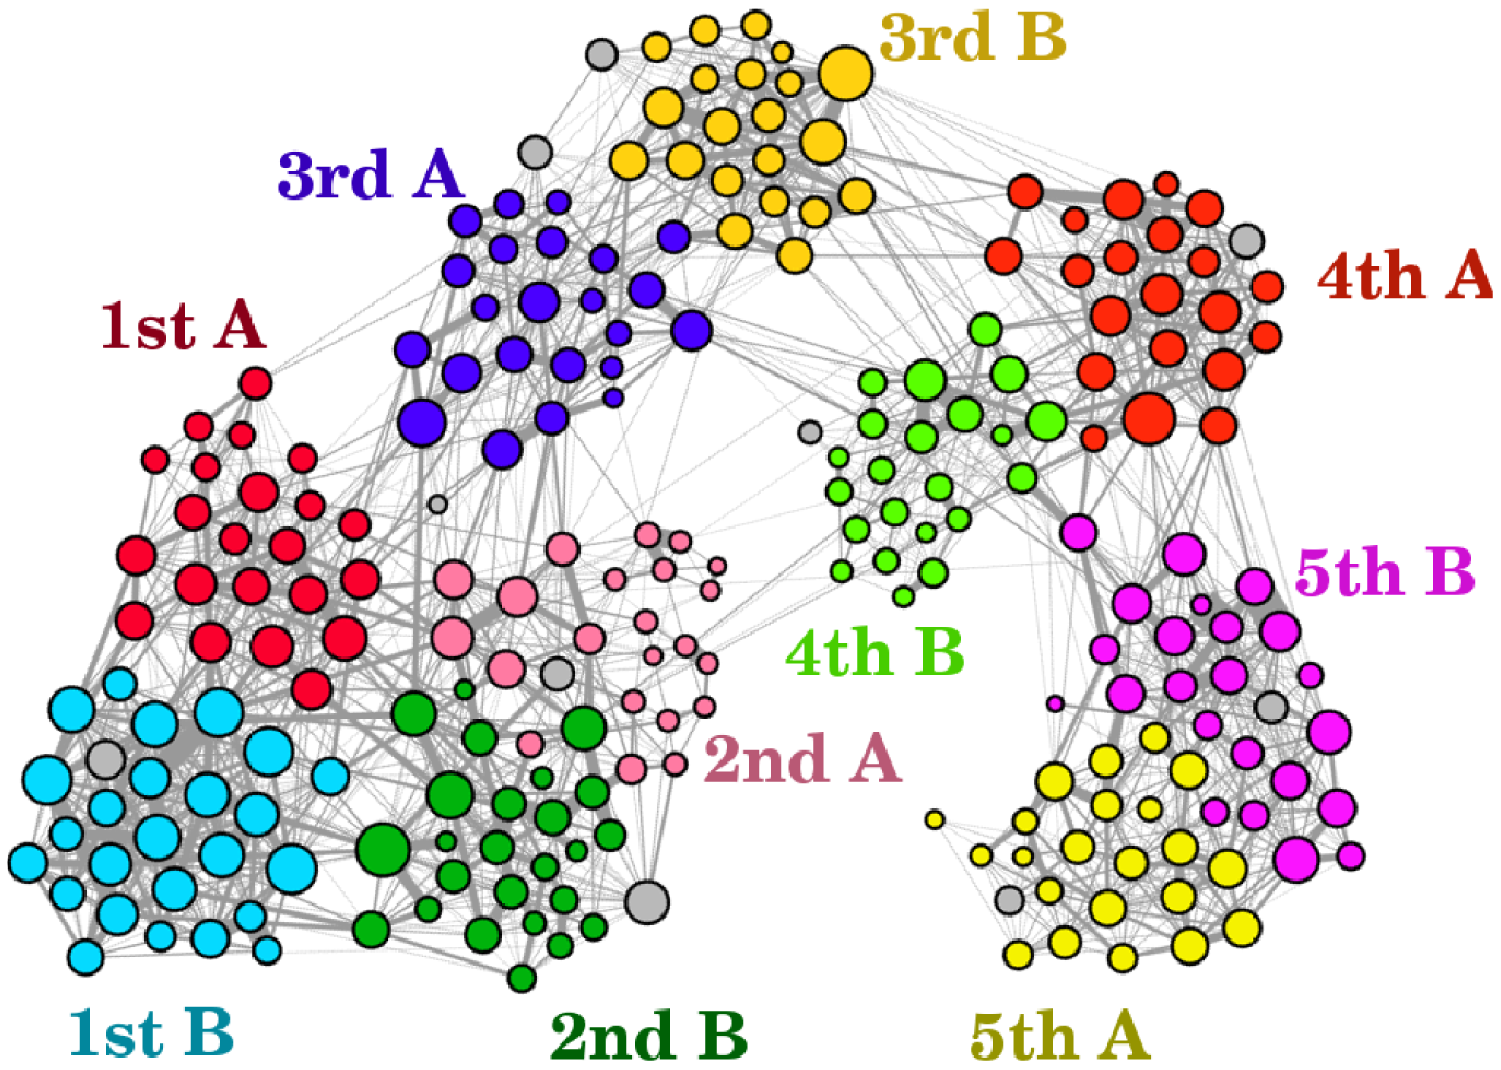
\includegraphics[width=0.7\linewidth]{img/Intro/ecole_primaire}
\caption{Graphe de contact des enfant d'une école primaire. L'épaisseur du lien représente la durée de communication entre deux élèves. La couleur représente la classe de chaque élèves. Les professeurs sont en gris.\protect\footnotemark}
\label{fig:ecole_primaire}
\end{figure}
\footnotetext{Image provenant de \url{http://journals.plos.org/plosone/article?id=10.1371/journal.pone.0023176}.}

Afin de capturer des partitions de n\oe uds, beaucoup de méthodes existent.
Il y a d'ailleurs régulièrement des état de l'art qui sont publiés~\cite{Fortunato2010,Plantie2013a, Malliaros2013a, Harenberg2014a}

limite modu: \cite{Fortunato2007,Good2010,Lancichinetti2011} extension \cite{Reichardt2006,Delvenne2010}, modu + vite \cite{Huang2015,Blondel2008a,Traag2015a}
modularité~\cite{Newman2004}, infomap\cite{Rosvall2008}, infomap hierachique\cite{Rosvall2011a}, limite infomap\cite{Kawamoto2015}, SBM \cite{Holland1983a}, LPA\cite{Raghavan2007a}, Surprise, méthode spectral
lien entre SBM et modularité\cite{Newman2016}


\subsection{Couverture de n\oe uds}
\label{subsec:cover}
Etat de l'art.
\cite{Danisch2012, Kanawati2014, Xie2013,Bandyopadhyay2015, Hric2014a}
Survey specific LPA\cite{Kanawati2014}.

infomap\cite{Esquivel2011},  MMSBM~\cite{Ball2011,Airoldi2008,Gopalan2013a} \cite{Yang2013} bigclam, OSLOM\cite{Lancichinetti2011a}, clique percolation\cite{Palla2005} fonction de qualité locale (conductance, cohésion), fonction de proximité
Demon \cite{Coscia2012c} LPA
\cite{Evans2009} evans, proche de evans \cite{Wang}, map equation\cite{Kim2011} tout ça avec ahn \cite{Ahn2010a} \cite{He2014}, \cite{Huang2013} \cite{Kim2014a} \cite{Lim2014} \cite{Shi2013}, \cite{Yu2013}.

extension modu: \cite{Shen2009,Nicosia2009}

\subsection{Comapraison}
ARI, NMI \cite{Danon2005}, futur nmi\cite{Zhang2015}, F1-score, Omega index. \cite{Porumbel2011}



benchmark \cite{Lancichinetti2008,Lancichinetti2009b}

\section{Extension temporelle des graphes}
\label{sec:intro_extension_temporelle}

\cite{Hartmann2014}

application:
Diffusions \cite{Backlund2014, Gauvin2015} \cite{Karimi2013,Holme2014a,Horvath2014,Karsai2011,Kivela2012,Lambiotte2013,Lee2012,Perotti2014,Rocha2011,Scholtes2014,Scholtes2013}temporal network \cite{Jo2014} impact inter event time
Face-to-face interaction: \cite{Barrat2013,Asur2009}
Communauté TVG: \cite{Bassett2013,Bazzi2016}
Réseau de transport: \ref{Gallotti2015} multilayer
\subsection{snapshot}
multylayer \cite{Mucha2010,Kivela2014,Peixoto2015c},mathemical source\cite{DeDomenico2013}, survey générale (génération, percolation, diffusion) \cite{Boccaletti2014}

snap\cite{Asur2009,Bassett2013,Bazzi2014} + fenetre glissante
\cite{de2016detection,Rosvall2010} change point snap

effet time window \cite{Krings2012,Ribeiro2013} (ribeiro effet sur les random walk)

centralité de lien \cite{Takaguchi2012}

Communauté:
\cite{Sun2007} graphescope
\cite{Lin2008} facenet
\cite{DeDomenico2014} info map sur du multi layer
\cite{Chakrabarti2006,Chen2013} current + stabilité
Multylayer SBM\cite{Stanley2015} \cite{Corneli2016} SBM sur chaque tranche. proche\cite{Matias2015}
\cite{Gauvin2014}
\cite{Guo2014}
\cite{Hopcroft2004}
\cite{Kalavathi2015}
temps intrinsèque.
\cite{Albano2014}

Génération de: \cite{Granell2015, Karsai2014,Perra2012}

\subsection{TVG/Evolving}
\cite{Casteigts2011,Wehmuth2014}
\cite{Figueiredo2012} random walk.
\cite{Cazabet2010} conductance sur TVG
Suivi dans les snapshot de la force d'une communauté: \cite{Du2015}
\cite{Caceres2013} time scale on temporal networks 
\cite{Cordeiro2016} évolution modularité
\cite{Epasto2015} le plus dense à un instant
\cite{Sun2014}

\subsection{Flots de liens}
\cite{Holme2013a,Holme2015b,Holme2015} plein d'étude possible
Formalisation algébric \cite{Batagelj2015}.
bursty \cite{Karsai2012a,Karsai2011,Moinet2015,Stehle2010} inter event time \cite{Kivela2014a}, \cite{Malmgren2008,Malmgren2009} heavy tail, \cite{Rocha2013}

motif \cite{Kovanen2011a,Kovanen2013}.
Le formalisme de flot de liens est défini plus en profondeur dans le chapitre~\ref{chap:def_flot}.
randomwalk\cite{Starnini2012b}

\cite{Gaumont2016}
centralité \cite{Costa2015,Kim2012, Pfitzner2013a, Praprotnik2015,Scholtes2015,Takaguchi2016}
densité \cite{Viard2014a}

generateur \cite{Starnini2013,Vestergaard2014}